\documentclass[assd_tp3_main.tex]{subfiles}

\begin{document}

\section{Conversores $\Sigma\Delta$}
\subsection{Moduladores $\Sigma\Delta$ de primer orden }
Recordamos dos características importantes del modulador:
\begin{itemize}
\item \textbf{Oversampling}: distribuye el ruido de cuantización 
\item \textbf{Noise shaping}: expulsa la mayoría del ruido que estaba dentro de la banda a frecuencias altas. 
\end{itemize}
A continuación se presentan diagramas en bloques del modulador $\Sigma\Delta$ de primer orden.
\begin{figure}[H]
\centering
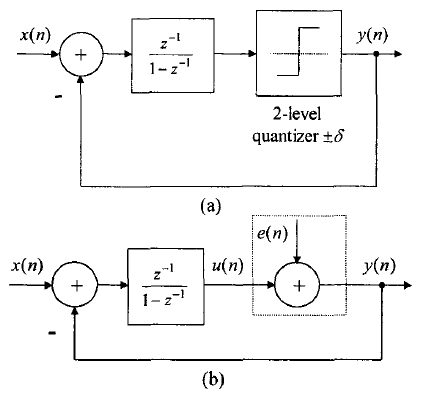
\includegraphics[width=0.4\linewidth]{images/ej4/sd_linmodel.png}
\caption{Diagrama en bloques del modulador $\Sigma\Delta$(a) y su modelo lineal(b)}
\label{fig:sigmadelmod_model}
\end{figure}
De la figura \ref{fig:sigmadelmod_model} obtenemos la SignalTransferFunction (STF) y la NoiseTransferFunction (NTF):
\[ Y(z)= z^{-1}X(z)+(1-z^{-1})E(z) \]
\[ STF(z)= z^{-1} \]
\[ NTF(z)= 1-z^{-1} \]


\end{document}
